
\documentclass[hyperref={pdfpagelabels=false},ngerman]{beamer}

% stop font warning
\let\Tiny=\tiny
\providecommand\thispdfpagelabel[1]{}

\usepackage[english]{babel}
\usepackage{lmodern}
\usepackage[T1]{fontenc}
\usepackage[utf8]{inputenc}
\usepackage{graphicx,import}
\usepackage{feynmp}
\DeclareGraphicsRule{*}{mps}{*}{} 
\DeclareGraphicsExtensions{.pdf}
\usepackage{amsmath,amssymb,amstext,amsfonts} % mathrsfs
\usepackage{array,booktabs,tabularx}
\usepackage{tikz,tikz-uml,pgf-pie}
\usetikzlibrary{shapes,calc,arrows,positioning}
\tikzstyle{block} = [rectangle, draw, text width=7em, text centered, minimum height=2em]
\tikzstyle{arrow} = [draw, -latex, thick]
\tikzstyle{arrow2} = [draw, latex-latex, thick]
\tikzstyle{quark}  = [rectangle, draw, fill=yellow, minimum width=2em, text centered, minimum height=2em]
\tikzstyle{lepton} = [rectangle, draw, fill=red!50, minimum width=2em, text centered, minimum height=2em]
\tikzstyle{gauge}  = [circle   , draw, fill=green , minimum size=2em, inner sep=0pt, text centered]
\tikzstyle{scalar} = [diamond  , draw, fill=blue!40, minimum width=2.3em, text centered, minimum height=2.3em, inner sep=0pt]
\tikzstyle{goldstone} = [diamond, draw, dashed, fill=blue!30, minimum width=2.3em, text centered, minimum height=2.3em, inner sep=0pt]
\tikzstyle{squark}   = [diamond, draw, fill=yellow, minimum width=2.3em, text centered, minimum height=2.3em, inner sep=0pt]
\tikzstyle{slepton}  = [diamond, draw, fill=red!50, minimum width=2.3em, text centered, minimum height=2.3em, inner sep=0pt]
\tikzstyle{gaugino}  = [rectangle, draw, fill=green , minimum size=2em, inner sep=0pt, text centered]
\tikzstyle{higgsino} = [rectangle, draw, fill=blue!40  , minimum width=2em, text centered, minimum height=2em]
\tikzstyle{inert}    = [diamond  , draw, fill=teal!80, minimum width=2.3em, text centered, minimum height=2.3em, inner sep=0pt]
\tikzstyle{inertino} = [rectangle, draw, fill=teal!80, minimum width=2em, text centered, minimum height=2em]
\tikzstyle{phantom}  = [rectangle, minimum width=2em, text centered, minimum height=2em]
\usepackage{slashed}
\usepackage{fixltx2e} % textsubscript
\usepackage{multirow}
\usepackage{tcolorbox}
\usepackage{pifont}
\usepackage{hyperref}
\hypersetup{colorlinks,linkcolor=,urlcolor=blue}
\usepackage{listings}
\lstset{breaklines=true,
  breakatwhitespace=true,
%  numbers=left,
  numberstyle=\tiny,
  stepnumber=1,
  basicstyle=\ttfamily\footnotesize,
  commentstyle=\ttfamily\color{gray},
  postbreak={\mbox{{$\hookrightarrow$}}\space\space},
  breakindent=10pt,
  breakautoindent=false,
  showspaces=false,
  showstringspaces=false,
  frame=single}

\definecolor{darkgreen}{RGB}{0,176,0}

\newcommand{\cmark}{\ding{51}}%
\newcommand{\xmark}{\ding{55}}%
\newcommand{\fmfvcenter}[1]{\;\vcenter{\hbox{\fmfreuse{#1}}}\;}
\newcommand{\eh}[1]{\,\mathsf{#1}}
\newcommand{\ok}{\textcolor{darkgreen}{\cmark}}
\newcommand{\notok}{\textcolor{red}{\xmark}}
\newcommand{\maybe}{\textcolor{gray}{\cmark}}
\newcommand{\Lagr}{\mathcal{L}}
\newcommand{\mathi}{\mathsf{i}}
\newcommand{\mycite}[1]{\textcolor{darkgray}{\tiny [#1]}}
\newcommand{\bigcite}[1]{\textcolor{darkgray}{[#1]}}
\newcommand{\dimrep}[1]{\mathbf{#1}}
\newcommand{\dimrepadj}[1]{\mathbf{\overline{#1}}}
\newcommand{\ESSM}{E\textsubscript{6}SSM}
\newcommand{\CESSM}{CE\textsubscript{6}SSM}
\DeclareMathOperator{\tildeRe}{\widetilde Re}
\DeclareMathOperator{\sign}{sign}
\DeclareMathOperator{\re}{Re}
\DeclareMathOperator{\im}{Im}
\renewcommand{\emph}{\textbf}
\newcommand{\dd}{\mathsf{d}}
\newcommand{\myurl}[1]{\href{#1}{#1}}
\newcommand{\Superpot}{\mathcal{W}}
\newcommand{\SuperField}[1]{#1}
\newcommand{\ConjSuperField}[1]{\bar{#1}}
\newcommand{\UY}{\ensuremath{U(1)_{Y}}}
\newcommand{\UN}{\ensuremath{U(1)_{N}}}
\newcommand{\Uem}{\ensuremath{U(1)_\text{em}}}
\newcommand{\SUL}{\ensuremath{SU(2)_\text{L}}}
\newcommand{\SUc}{\ensuremath{SU(3)_\text{c}}}
\newcommand{\SOten}{\ensuremath{{SO(10)}}}
\newcommand{\comma}{,}
\newcommand{\DRbar}{\ensuremath{\overline{\text{DR}}}}
\newcommand{\MSbar}{\ensuremath{\overline{\text{MS}}}}
\newcommand{\SM}{\ensuremath{\text{SM}}}
\newcommand{\MSSM}{\ensuremath{\text{MSSM}}}
\newcommand{\pole}{\ensuremath{\text{pole}}}
\newcommand{\tree}{\ensuremath{\text{tree}}}
\newcommand{\Zv}{\ensuremath{\backslash\mkern-11.0mu{Z_3}}}
\newcommand{\downrightknickarrow}{\mathrel{\scalebox{1.3}{\rotatebox[origin=c]{180}{$\Lsh$}}}}
\newcommand{\threelinebrace}{$\left. \begin{array}{c} \\ \\ \\ \end{array} \right\rbrace$}
\newcommand{\fivelinebrace}{$\left. \begin{array}{c} \\ \\ \\ \\ \\ \end{array} \right\rbrace$}
\newcommand{\twolinebrace}{$\left. \begin{array}{c} \\ \\ \end{array} \right\rbrace$}
\newcommand{\elevenlinebrace}{$\left. \begin{array}{c} \\ \\ \\ \\ \\ \\ \\ \\ \\ \\ \\ \end{array} \right\rbrace$}

% set look of slides
\usetheme{Madrid}
\useoutertheme{default}
\useinnertheme{circles}
\usecolortheme{default}
\beamertemplatenavigationsymbolsempty % keine Navigationselemente
\setbeamersize{text margin left = 1cm, text margin right = 1cm}

% define footer
\makeatletter
\setbeamertemplate{footline}
{
  \hfill\hbox{\insertframenumber{} / \inserttotalframenumber\hspace*{4pt}}%
  \vskip3pt%
}
\makeatother
\usecolortheme{tud}

\title{Automated Higgs mass prediction in BSM models with
  FlexibleSUSY using a mixed diagrammatic / EFT approach}

\author[Alexander Voigt]{Tom Steudtner, Dominik Stöckinger, \underline{Alexander Voigt}}

\date{20.01.2016}

\institute[Heidelberg]{KUTS 2016 Heidelberg}
\subject{FlexibleSUSY,MSSM,Higgs}
\keywords{FlexibleSUSY,MSSM,Higgs}

%%%%%%%%%%%%%%%%%%%%%%%%%%%%%%%%%%%%%%%%%%%%%%%%%%%%%%%%%%%%%%%%%%%%%%%%%%%%%

\begin{document}

\section{What is FlexibleSUSY?}

%%%%%%%%%%%%%%%%%%%%%%%%%%%%%%%%%%%%%%%%
\begin{frame}[plain]
  \tikz [remember picture,overlay]
  \node at
    ([yshift=1.3cm,xshift=5cm]current page.south)
    {
\includegraphics[height=2cm]{images/DESY_Logo}};
  \titlepage  
  % \vspace*{1em}
  % \centering In collaboration with Peter Athron, Jae-hyeon Park and Dominik Stöckinger [\href{https://arxiv.org/abs/1406.2319}{arxiv:1406:2319}] 
\end{frame}

%%%%%%%%%%%%%%%%%%%%%%%%%%%%%%%%%%%%%%%%
\begin{frame}
  \frametitle{Contents}
  \tableofcontents
\end{frame}

\begin{frame}{FlexibleSUSY = spectrum generator generator}
  \begin{center}
    FlexibleSUSY~~~~~\\
    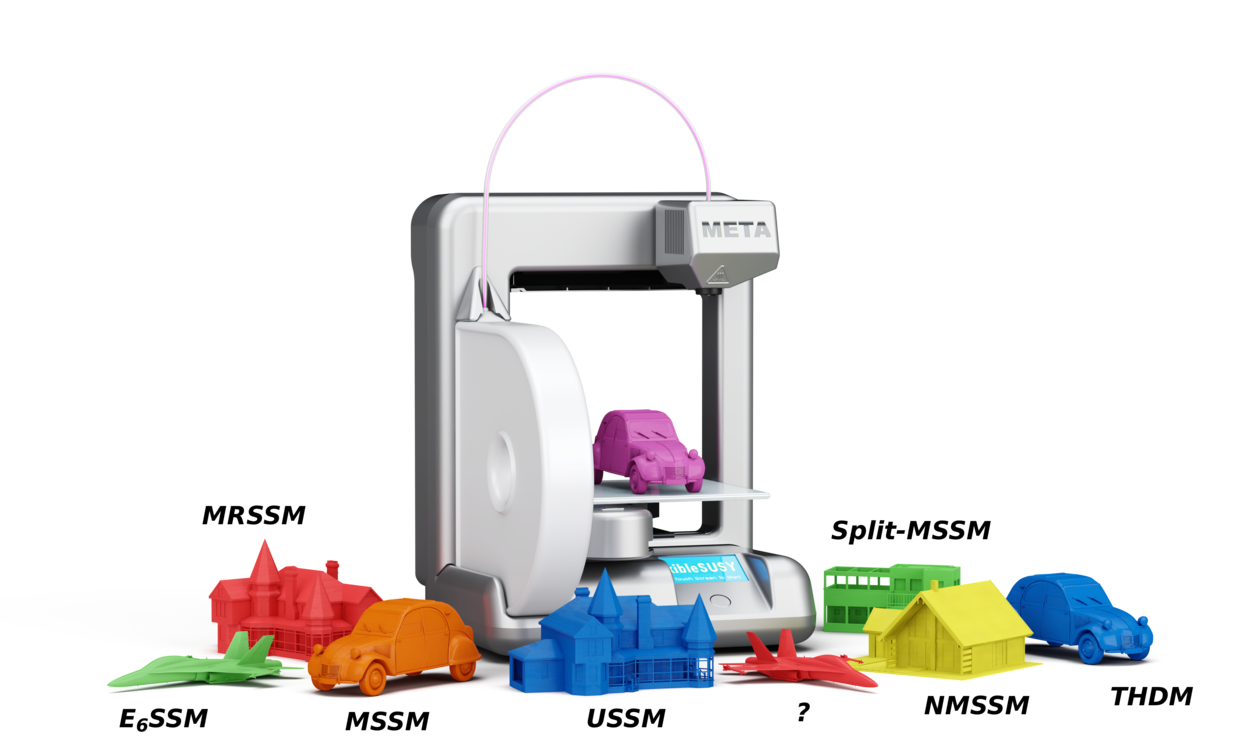
\includegraphics[width=\textwidth]{images/FS.png}
  \end{center}
\end{frame}

\begin{frame}{Generating a spectrum generator}
  \begin{figure}
    \centering
    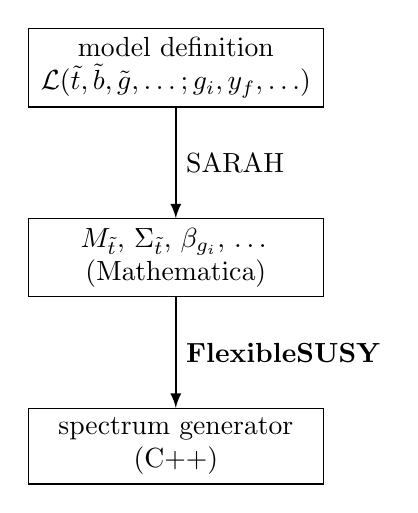
\begin{tikzpicture}[node distance=4em]
      \node [block, text width=10em] (Lagr) {model definition\\ $\Lagr(\tilde t, \tilde b, \tilde g,\ldots; g_i, y_f,\ldots)$};
      \node [block, below=of Lagr, text width=10em] (expr1) {$M_{\tilde t}$, $\Sigma_{\tilde t}$, $\beta_{g_i}$,
        \ldots\\ (Mathematica)};
      \node [block, below=of expr1, text width=10em] (flexiblesusy) {spectrum generator\\(C++)};
      \path [arrow] (Lagr) -- node[right] {SARAH} (expr1);
      \path [arrow] (expr1) -- node[right] {\emph{FlexibleSUSY}} (flexiblesusy);
    \end{tikzpicture}
  \end{figure}
\end{frame}

\section{Available models}

%%%%%%%%%%%%%%%%%%%%%%%%%%%%%%%%%%%%%%%%

\begin{frame}{Available models (selection)}
  \begin{table}
    \centering
    \begin{tabular}{llll}
      Model             & RGEs & \multicolumn{2}{l}{diagrammatic $M_h$ contributions} \\
      \midrule
      MSSM              & 3L   & \multicolumn{2}{l}{1L + 2L $O((\alpha_t + \alpha_b) \alpha_s + (\alpha_t + \alpha_b)^2)$} \\
      NMSSM             & 2L   & \multicolumn{2}{l}{1L + 2L $O((\alpha_t + \alpha_b) \alpha_s + (\alpha_t + \alpha_b)^2)$} \\
      USSM              & 2L   & \multicolumn{2}{l}{1L + 2L $O((\alpha_t + \alpha_b) \alpha_s + (\alpha_t + \alpha_b)^2)$} \\
      E6SSM             & 2L   & \multicolumn{2}{l}{1L + 2L $O((\alpha_t + \alpha_b) \alpha_s + (\alpha_t + \alpha_b)^2)$} \\
      THDM              & 2L   & 1L \\
      THDM + $\tilde{h}_i$ & 2L   & 1L \\
      THDM + split      & 2L   & 1L \\
    \end{tabular}
  \end{table}
\end{frame}

%%%%%%%%%%%%%%%%%%%%%%%%%%%%%%%%%%%%%%%%

\begin{frame}{Available models matched to the MSSM at $M_S$}
  \resizebox{\textwidth}{!}{%
    \begin{tabular}{llll}
      Model             & RGEs & diagrammatic $M_h$ & matching \\
                        &      & contributions      & conditions \\
      \midrule
      SM + split        & 2L   & 1L + 2L $O(\alpha_t (\alpha_s + \alpha_t))$       & 1L $\tilde{g}_{ij}$ $O(\alpha_t + \alpha_i)$ \\
                        &      & \phantom{1L} + 3L gluino $O(\alpha_t \alpha_s^2)$ & + 1L $\lambda$ $O((\alpha_t + \alpha_i)^2)$ \\
                        &      &                                                  & + 2L $\lambda$ $O(\alpha_s \alpha_t^2)$ \\
                        &      &                                                  & \mycite{1407.4081} \\[0.5em]
      SM                & 3L   & 1L + 2L $O(\alpha_t (\alpha_s + \alpha_t))$ & 1L $\lambda$ $O((\alpha_t + \alpha_i)^2 + \alpha_b^2 + \alpha_\tau^2)$ \\
      ($\approx$ SUSYHD) &      &                                            & 2L $\lambda$ $O((\alpha_s + \alpha_t)\alpha_t^2)$ \\
                        &      &                                            & \mycite{1407.4081, 1504.05200} \\[0.5em]
      SM                & 3L   & 1L + 2L $O(\alpha_t (\alpha_s + \alpha_t))$ & 1L $\lambda$ + $p^2/M_S^2$ terms \\
    \end{tabular}}
\end{frame}

%%%%%%%%%%%%%%%%%%%%%%%%%%%%%%%%%%%%%%%%

\begin{frame}{Tower of EFTs}
  \begin{figure}
    \centering
    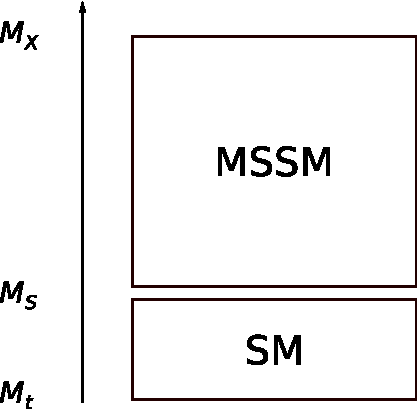
\includegraphics[width=0.6\textwidth]{images/mssm-sm-tower}
  \end{figure}
\end{frame}

%%%%%%%%%%%%%%%%%%%%%%%%%%%%%%%%%%%%%%%%

\begin{frame}{Different approaches}
  \begin{minipage}[t]{0.45\textwidth}
    \centering
    Diagrammatic approach\\[1em]
    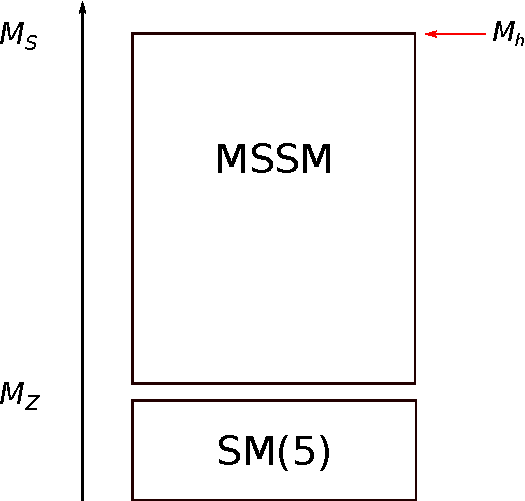
\includegraphics[width=\textwidth]{images/mssm-sm-tower-diagrammatic}
  \end{minipage}
  \hfill
  \begin{minipage}[t]{0.45\textwidth}
    \centering
    EFT approach\\[1em]
    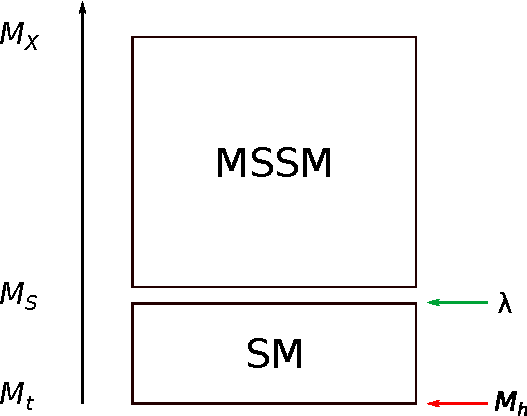
\includegraphics[width=\textwidth]{images/mssm-sm-tower-eft}
  \end{minipage}
\end{frame}

\begin{frame}{Diagrammatic approach (\DRbar\ codes)}
  \begin{center}
    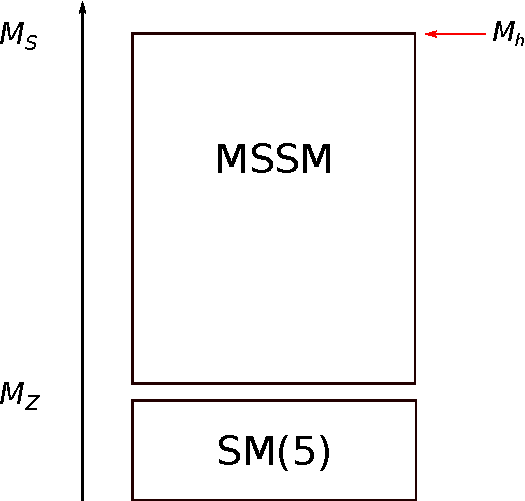
\includegraphics[width=0.45\textwidth]{images/mssm-sm-tower-diagrammatic}\\[1em]
  \end{center}
  \emph{Idea:} Calculate $M_h$ in the MSSM as a function of the \DRbar\ parameters:\\[1em]
  \centering $g_i$, $y^f_{ij}$, $v_i$, $\mu$, $B\mu$, $m^2_{H_i}$,
  $m_{\tilde{f},ij}^2$, $M_i$, $T^f_{ij}$
\end{frame}

\begin{frame}{Diagrammatic approach (\DRbar\ codes)}
  \emph{Fixed by observables:}
  \begin{table}
    \centering
    \begin{tabular}{lllll}
      Input & & & & Output \\
      \midrule
      $\alpha_\text{em}^{\SM(5)}(M_t)$ & $\rightarrow$ & $e^\MSSM(M_t)$ & $\rightarrow$ & $g_1^\MSSM(M_t)$ \\
      $G_F$ & $\rightarrow$ & $\sin\theta_W^\MSSM(M_t)$ & $\rightarrow$ & $g_2^\MSSM(M_t)$ \\
      $\alpha_\text{s}^{\SM(5)}(M_t)$ & & & $\rightarrow$ & $g_3^\MSSM(M_t)$ \\
      $M_Z$ & $\rightarrow$ & $m_Z^\MSSM(M_t)$ & $\rightarrow$ & $v^\MSSM(M_t)$ \\
      $M_t$ & $\rightarrow$ & $m_t^\MSSM(M_t)$ & $\rightarrow$ & $y_t^\MSSM(M_t)$ \\
      $m_b^{\SM(5)}(m_b)$ & $\rightarrow$ & $m_b^\MSSM(M_t)$ & $\rightarrow$ & $y_b^\MSSM(M_t)$ \\
      $M_\tau$ & $\rightarrow$ & $m_\tau^\MSSM(M_t)$ & $\rightarrow$ & $y_\tau^\MSSM(M_t)$ \\
    \end{tabular}
  \end{table}
  \emph{Fixed by 2 EWSB conditions:} $m^2_{H_u}$, $m^2_{H_d}$ \\[1em]
  \emph{Free parameters:} $\tan\beta$, $\mu$, $B\mu$, $m_{\tilde{f},ij}^2$, $M_i$,
  $T^f_{ij}$
\end{frame}

\begin{frame}{Diagrammatic approach (\DRbar\ codes)}
  \begin{align*}
    (M_h^\text{MSSM})^2 &= \text{smallest eigenvalue of} \\
    &\phantom{={}} \left[(m_h^\text{MSSM})^2 - \Sigma^\text{MSSM}_h(p^2 = (M_h^\text{MSSM})^2,\mu = M_S)\right]_{ij}
  \end{align*}
  \emph{Advantage:} includes terms $O(p^2/M_S^2)$\\
  \emph{Disadvantage:} suffers from large logarithms $\log(M_t/M_S)$\\
\end{frame}

%%%%%%%%%%%%%%%%%%%%%%%%%%%%%%%%%%%%%%%%

\begin{frame}{EFT approach}
  \begin{center}
    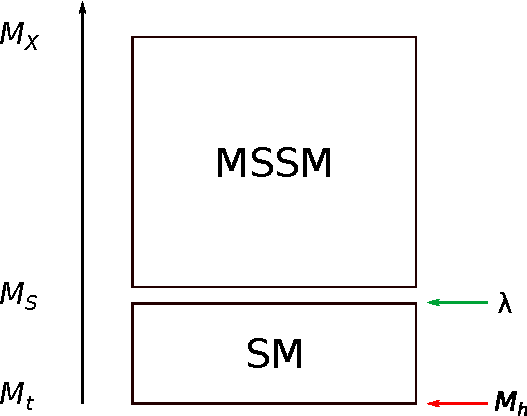
\includegraphics[width=0.45\textwidth]{images/mssm-sm-tower-eft}\\[1em]
  \end{center}
  \emph{Idea:} Calculate $M_h$ in the SM as a function of the \MSbar\ parameters:\\[1em]
  \centering $g_i$, $y^f_{ij}$, $v$, $\mu^2$, $\lambda$
\end{frame}

\begin{frame}{EFT approach}
  \emph{Fixed by observables:}
  \begin{table}
    \centering
    \begin{tabular}{lllll}
      Input & & & & Output \\
      \midrule
      $\alpha_\text{em}^{\SM(5)}(M_t)$ & $\rightarrow$ & $e^\SM(M_t)$ & $\rightarrow$ & $g_1^\SM(M_t)$ \\
      $G_F$ & $\rightarrow$ & $\sin\theta_W^\SM(M_t)$ & $\rightarrow$ & $g_2^\SM(M_t)$ \\
      $\alpha_\text{s}^{\SM(5)}(M_t)$ & & & $\rightarrow$ & $g_3^\SM(M_t)$ \\
      $M_Z$ & $\rightarrow$ & $m_Z^\SM(M_t)$ & $\rightarrow$ & $v^\SM(M_t)$ \\
      $M_t$ & $\rightarrow$ & $m_t^\SM(M_t)$ & $\rightarrow$ & $y_t^\SM(M_t)$ \\
      $m_b^{\SM(5)}(m_b)$ & $\rightarrow$ & $m_b^\SM(M_t)$ & $\rightarrow$ & $y_b^\SM(M_t)$ \\
      $M_\tau$ & $\rightarrow$ & $m_\tau^\SM(M_t)$ & $\rightarrow$ & $y_\tau^\SM(M_t)$ \\
    \end{tabular}
  \end{table}
  \emph{Fixed by 1 EWSB condition:} $\mu^2$ \\[1em]
  \emph{Free parameter:} $\lambda$
\end{frame}

\begin{frame}{EFT approach: matching all $\Gamma_{\phi_1,\ldots,\phi_n}$}
  Determine $\lambda(M_S)$ from mathching all $\Gamma_{\phi_1,\ldots,\phi_n}$:
  \begin{align*}
    \frac{\partial}{\partial p^2}\Gamma_{hh}^{\SM}(p^2 = 0, \mu = M_S) &= \frac{\partial}{\partial p^2}\Gamma_{hh}^\text{MSSM}(p^2 = 0, \mu = M_S) \\
    \Gamma_{hhhh}^{\SM}(p^2 = 0, \mu = M_S) &= \Gamma_{hhhh}^\text{MSSM}(p^2 = 0, \mu = M_S)
  \end{align*}
  $\Rightarrow$
  \begin{align*}
    \lambda (M_S) &= \frac{1}{4}\left[\frac{3}{5} g_1^{2} + g_2^2\right] \cos^22\beta
    + \Delta \lambda
  \end{align*}
  $\Rightarrow$
  \begin{align*}
    (M_h^\SM)^2 &= (m_h^\SM)^2 - \Sigma^\SM_h(p^2 = (M_h^\SM)^2,\mu =
    M_t)
  \end{align*}
  \emph{Advantage:} resums large logarithms $\log(M_Z/M_S)$\\
  \emph{Disadvantage:} neglects terms $O(p^2/M_S^2)$
\end{frame}

%%%%%%%%%%%%%%%%%%%%%%%%%%%%%%%%%%%%%%%%

\begin{frame}{Combining EFT and diagrammatic approach}
  \begin{center}
    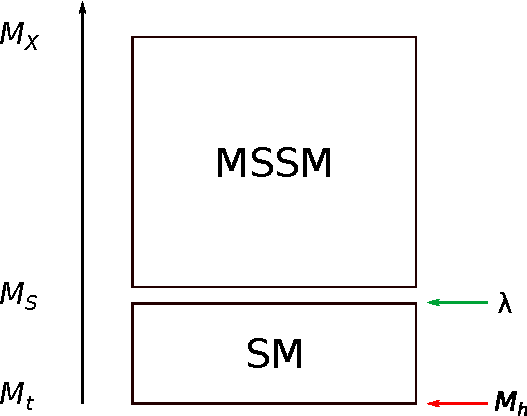
\includegraphics[width=0.45\textwidth]{images/mssm-sm-tower-eft}\\[1em]
  \end{center}
  \emph{Idea:} Calculate $M_h$ in the SM as a function of the \MSbar\ parameters:\\[1em]
  \begin{center}
    $g_i$, $y^f_{ij}$, $v$, $\mu^2$, $\lambda$
  \end{center}
  \emph{including terms $O(p^2/M_S^2)$}
\end{frame}

\begin{frame}{Combining EFT and diagrammatic approach: matching $M_h$}
  \begin{align*}
    M_h^{\SM} &= M_h^\text{MSSM}
  \end{align*}
  $\Rightarrow$
  \begin{align*}
    \lambda_{n+1} \leftarrow \frac{1}{v^2} \left[ (M_h^\text{MSSM})^2 - (M_h^{\SM})^2 + \lambda_n v^2 \right]
  \end{align*}
  where
  \begin{align*}
    (M_h^{\SM})^2 &= \lambda_n v^2 - \Sigma^{\SM}_h(p^2 = (M_h^{\SM})^2,\mu = M_S) \\
    (M_h^\text{MSSM})^2 &= \text{smallest eigenvalue of} \\
    &\phantom{={}} \left[(m_h^\text{MSSM})^2 - \Sigma^\text{MSSM}_h(p^2 = (M_h^\text{MSSM})^2,\mu = M_S)\right]_{ij}
  \end{align*}
  \emph{Advantage:} resums large logarithms $\log(M_Z/M_S)$\\
  \emph{Advantage:} includes 1L terms $O(p^2/M_S^2)$
\end{frame}

%%%%%%%%%%%%%%%%%%%%%%%%%%%%%%%%%%%%%%%%

\begin{frame}{Comparison fixed order / EFT}
  \begin{figure}
    \centering
    \includegraphics[width=\textwidth]{plots/PlotScale-in-FH_new_low-selected}
  \end{figure}
  $\tan\beta = 5$, $X_{t,b,\tau} = 0$
\end{frame}

%%%%%%%%%%%%%%%%%%%%%%%%%%%%%%%%%%%%%%%%

\begin{frame}{Comparison fixed order / EFT}
  \begin{figure}
    \centering
    \includegraphics[width=\textwidth]{plots/PlotXt-selected}
  \end{figure}
  $\tan\beta = 5$, $X_{b,\tau} = 0$, $M_S = 2\eh{TeV}$
\end{frame}

%%%%%%%%%%%%%%%%%%%%%%%%%%%%%%%%%%%%%%%%

\begin{frame}{NMSSM variants available in FlexibleSUSY}
  $Z_3$-symmetric NMSSM (called \texttt{NMSSM} in FlexibleSUSY):
  \begin{align*} 
    W_{Z_3} &= y_e (H_d L) \bar{E}
      + y_d (H_d Q) \bar{D}
      + y_u (Q H_u) \bar{U}\\
      &\phantom{={}}
      \textcolor{blue}{+ \lambda S (H_d H_u) + \frac{\kappa}{3}S^{3}} \\
    \Lagr_{\text{soft},Z_3} &= \Lagr_\text{soft,MSSM}(B\mu=0)\\
    &\phantom{={}}
    \textcolor{blue}{ -\ m_s^2|s|^2 
      -\left(\lambda A_\lambda s (h_d h_u)
        + \frac{\kappa A_\kappa}{3} s^3 + \text{h.c.}\right)}
  \end{align*}
\end{frame}

\begin{frame}{NMSSM variants available in FlexibleSUSY}
  $\Zv$-NMSSM (called \texttt{SMSSM} in FlexibleSUSY):
  \begin{align*} 
    W_{\Zv} &= y_e (H_d L) \bar{E}
      + y_d (H_d Q) \bar{D}
      + y_u (Q H_u) \bar{U}\\
      &\phantom{={}}
      \textcolor{blue}{+ \lambda S (H_d H_u) + \frac{\kappa}{3}S^{3}} \\
      &\phantom{={}}
      \textcolor{red}{+ \mu(H_d H_u) + \xi_FS 
      + \frac{\mu^\prime}{2} S^{2}}\\
    \Lagr_{\text{soft},\Zv} &= \Lagr_\text{soft,MSSM}(B\mu=0)\\
    &\phantom{={}}
    \textcolor{blue}{ -\ m_s^2|s|^2 
      -\left(\lambda A_\lambda s (h_d h_u)
        + \frac{\kappa A_\kappa}{3} s^3 + \text{h.c.}\right)}\\
    &\phantom{={}}
    \textcolor{red}{ -\ \xi_s s - \frac{m_s^{\prime \, 2}}{2} s^2
    - B\mu (h_d h_u) + \text{h.c.}}
  \end{align*}
\end{frame}

\subsection{Parameters}

%%%%%%%%%%%%%%%%%%%%%%%%%%%%%%%%%%%%%%%%
\begin{frame}{NMSSM parameters ($\DRbar$ scheme)}
  \begin{table}[tbh]
    \footnotesize
    \centering
    \begin{tabularx}{\textwidth}{lXX}
      \toprule
      & $Z_3$ (\texttt{NMSSM}) & $\Zv$ (\texttt{SMSSM})\\
      \midrule
      fixed by SM
      & $g_Y$, $g_2$, $g_3$, $y_u$, $y_d$, $y_e$, $v_u$, $v_d$
      & $g_Y$, $g_2$, $g_3$, $y_u$, $y_d$, $y_e$, $v_u$, $v_d$
      \\\midrule
      fixed by EWSB
      & $\kappa$, $|v_s|$, $m_s^2$
      & $|\mu|^2$, $B\mu$, $\xi_s$
      \\\midrule
      User input
      & $m_q^2$, $m_u^2$,  $m_d^2$, $m_\ell^2$, $m_e^2$,
      & $m_q^2$, $m_u^2$,  $m_d^2$, $m_\ell^2$, $m_e^2$,\\
      (general)
      & $m_{h_d}^2$, $m_{h_u}^2$,
      & $m_{h_d}^2$, $m_{h_u}^2$, $m_s^2$,\\
      & $A_e$, $A_d$, $A_u$, $A_\lambda$, $A_\kappa$,
      & $A_e$, $A_d$, $A_u$, $A_\lambda$, $A_\kappa$,
      \\
      & $M_1$, $M_2$, $M_3$,
      & $M_1$, $M_2$, $M_3$,
      \\
      & $\lambda$, $\sign v_s$
      & $\lambda$, $\sign\mu$,
      \\
      & & $\kappa$, $v_s$, $\mu'$, $m_s^{\prime 2}$, $\xi_F$
      % \\\midrule
      % User input
      % & $m_0^2$, $A_0$, $M_{1/2}$,
      % & $m_0^2$, $A_0$, $M_{1/2}$,
      % \\
      % (mSUGRA)
      % & $\lambda$, $\tan\beta$, $\sign v_s$
      % & $\lambda$, $\tan\beta$, $\sign\mu$,\\
      % & &
      % $\kappa$, $v_s$, $m_s^2$, $\mu'$, $m_s^{\prime 2}$, $\xi_F$
      \\\bottomrule
    \end{tabularx}
  \end{table}
\end{frame}

%%%%%%%%%%%%%%%%%%%%%%%%%%%%%%%%%%%%%%%%
\begin{frame}{NMSSM parameters ($\DRbar$ scheme)}
  \begin{table}[tbh]
    \footnotesize
    \centering
    \begin{tabularx}{\textwidth}{lXX}
      \toprule
      & $Z_3$ (\texttt{NUTNMSSM}) & $\Zv$ (\texttt{NUTSMSSM})\\
      \midrule
      fixed by SM
      & $g_Y$, $g_2$, $g_3$, $y_u$, $y_d$, $y_e$, $v_u$, $v_d$
      & $g_Y$, $g_2$, $g_3$, $y_u$, $y_d$, $y_e$, $v_u$, $v_d$
      \\\midrule
      fixed by EWSB
      & \textcolor{darkgreen}{$m_{h_d}^2$, $m_{h_u}^2$}, $m_s^2$
      & \textcolor{darkgreen}{$m_{h_d}^2$, $m_{h_u}^2$, $m_s^2$}
      \\\midrule
      User input
      & $m_q^2$, $m_u^2$,  $m_d^2$, $m_\ell^2$, $m_e^2$,
      & $m_q^2$, $m_u^2$,  $m_d^2$, $m_\ell^2$, $m_e^2$,\\
      (general)
      & \textcolor{darkgreen}{$\kappa$, $|v_s|$},
      & \textcolor{darkgreen}{$|\mu|^2$, $B\mu$, $\xi_s$},\\
      & $A_e$, $A_d$, $A_u$, $A_\lambda$, $A_\kappa$,
      & $A_e$, $A_d$, $A_u$, $A_\lambda$, $A_\kappa$,
      \\
      & $M_1$, $M_2$, $M_3$,
      & $M_1$, $M_2$, $M_3$,
      \\
      & $\lambda$, $\sign v_s$
      & $\lambda$, $\sign\mu$,
      \\
      & & $\kappa$, $v_s$, $\mu'$, $m_s^{\prime 2}$, $\xi_F$
      % \\\midrule
      % User input
      % & $m_0^2$, $A_0$, $M_{1/2}$,
      % & $m_0^2$, $A_0$, $M_{1/2}$,
      % \\
      % (mSUGRA)
      % & $\lambda$, $\tan\beta$, $\sign v_s$
      % & $\lambda$, $\tan\beta$, $\sign\mu$,\\
      % & &
      % $\kappa$, $v_s$, $m_s^2$, $\mu'$, $m_s^{\prime 2}$, $\xi_F$
      \\\bottomrule
    \end{tabularx}
  \end{table}
\end{frame}

\section{Physical problem statement}

\begin{frame}{Physical problem statement for the $Z_3$-NMSSM}
  \begin{figure}[tbh]
    \centering
    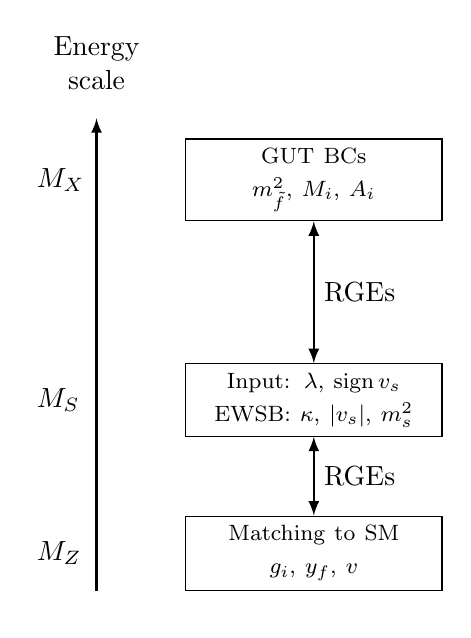
\begin{tikzpicture}[node distance = 3.5cm, auto]
      \node [block, text width=8.6em] (lowscale) {\footnotesize Matching to SM\\ $g_i$, $y_f$, $v$};
      \node [block, above=1cm of lowscale, text width=8.6em] (susyscale) {\footnotesize Input: $\lambda$, $\sign v_s$\\EWSB: $\kappa$, $|v_s|$, $m_s^2$};
      \node [block, above=1.8cm of susyscale, text width=8.6em] (highscale) {\footnotesize GUT BCs\\ $m_{\tilde{f}}^2$, $M_i$, $A_i$};
      \path [arrow2] (highscale) -- node (RGEs) {RGEs} (susyscale);
      \path [arrow2] (susyscale) -- node {RGEs} (lowscale);
      % energy axis
      \node [below left=0em and 1cm of lowscale] (energy_start) {};
      \node [above=6cm of energy_start] (energy_stop) {};
      \node [above=0em of energy_stop,align=center] (energy_label) {Energy \\ scale};
      \path [arrow] (energy_start) -- (energy_stop);
      \node [text width=2em,left=3.0em of highscale] (mx) {$M_X$};
      \node [text width=2em,left=3.0em of susyscale] (ms) {$M_S$};
      \node [text width=2em,left=3.0em of lowscale] (mz) {$M_Z$};
    \end{tikzpicture}
  \end{figure}
\end{frame}

\section{Algorithm to calculate the model parameters}

\begin{frame}{Algorithm to calculate the model parameters consistent with all BCs}
  \begin{figure}[tbh]
    \centering
    \small
    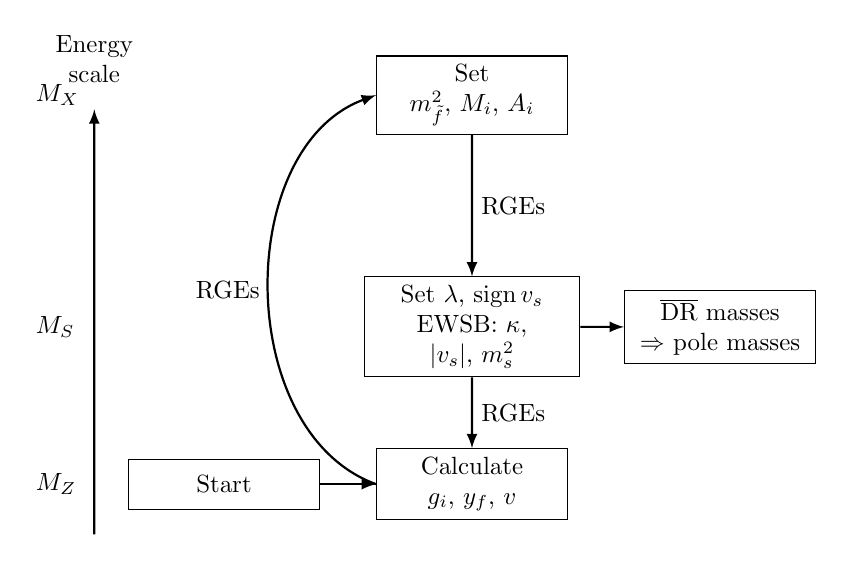
\begin{tikzpicture}[node distance = 3.5cm, auto,scale=0.9, every node/.style={transform shape}]
      \node [block] (guess) {Start};
      \node [block, right of=guess] (lowscale) {Calculate\\ $g_i$, $y_f$, $v$};
      \node [block, above=1cm of lowscale,text width=8em] (susyscale) {Set $\lambda$, $\sign v_s$\\EWSB: $\kappa$, $|v_s|$, $m_s^2$};
      \node [block, above=2cm of susyscale] (highscale) {Set\\ $m_{\tilde{f}}^2$, $M_i$, $A_i$};
      \node [block, right of=susyscale] (spec) {\DRbar\ masses\\ $\Rightarrow$ pole masses};
      \path [arrow] (guess) -- (lowscale);
      \path [-latex, thick] (lowscale.west) edge[bend left=70] node {RGEs} (highscale.west);
      \path [arrow] (highscale) -- node {RGEs} (susyscale);
      \path [arrow] (susyscale) -- node {RGEs} (lowscale);
      \path [arrow] (susyscale) -- (spec);
      % energy axis
      \node [below left=1em and 1em of guess] (energy_start) {};
      \node [above=6cm of energy_start] (energy_stop) {};
      \node [above=0em of energy_stop,align=center] (energy_label) {Energy\\ scale};
      \path [arrow] (energy_start) -- (energy_stop);
      \node [text width=3.3em,left=10em of highscale] (mx) {$M_X$};
      \node [text width=3.3em,left=9.5em of susyscale] (ms) {$M_S$};
      \node [text width=3.3em,left=10em of lowscale] (mz) {$M_Z$};
    \end{tikzpicture}
  \end{figure}
\end{frame}

\begin{frame}{Calculation of $g_3^{\DRbar}(M_Z)$}
  \emph{Input:} \ \ $\alpha_{\text{s},\text{SM}}^{(5),\text{\MSbar}}(M_Z) = 0.1185$\\[1em]
  $\rightarrow$
  \begin{align*}
    \alpha_{\text{s}}^{\text{\DRbar}}(M_Z) &=
    \frac{\alpha_{\text{s},\text{SM}}^{(5),\text{\MSbar}}(M_Z)}{1 -
      \Delta\alpha_{\text{s},\text{SM}}(M_Z)
      - \Delta\alpha_{\text{s}}(M_Z)}
    \intertext{with}
    \Delta\alpha_{\text{s},\text{SM}}(\mu) &=
    \frac{\alpha_\text{s}}{2\pi} \left[
      -\frac{2}{3} \log{\frac{m_t}{\mu}} \right]\\
    \Delta\alpha_{\text{s}}(\mu) &=
    \frac{\alpha_\text{s}}{2\pi}\left[ \frac{1}{2}-\sum_{\text{SUSY
          particle } f} T_f \log{\frac{m_f}{\mu}} \right]
    \intertext{$\Rightarrow$}
    g_{3}^{\text{\DRbar}}(M_Z) &=
    \sqrt{4\pi\alpha_{\text{s}}^{\text{\DRbar}}(M_Z)}
  \end{align*}
\end{frame}

\begin{frame}{Calculation of $y_t^{\DRbar}(M_Z)$}
  \begin{align*}
    y_t^{\DRbar}(M_Z) &= \frac{\sqrt{2}\,
      m_{t}^{\text{\DRbar}}(M_Z)}{v_u(M_Z)}
    %
    \intertext{where the running top mass is calculated from the pole
      mass $M_t$ as}
    %
    m_{t}^{\text{\DRbar}}(\mu) &= M_t +
    \re\Sigma_{t}^{S}(M_t) + M_t \Big[ \re\Sigma_{t}^{L}(M_t) \\
    &\phantom{={}} +
    \re\Sigma_{t}^{R}(M_t) + \Delta
    m_t^{(1),\text{gluon}} + \Delta m_t^{(2),\text{gluon}} \Big]\\
    % m_{t}^{\text{\DRbar}} &= M_t +
    % \Sigma_{t}^\text{no gluon}(M_t) + M_t \Big[\Delta
    % m_t^{(1L),\text{gluon}} + \Delta m_t^{(2L),\text{gluon}} \Big]
    % \\
    \Delta m_t^{(1L),\text{gluon}} &= -\frac{g_3^2}{12 \pi^2}
    \left[5-3 \log\left(\frac{m_t^2}{\mu^2}\right)\right]
    \\
    \Delta m_t^{(2L),\text{gluon}} &= \left(\Delta
      m_t^{(1L),\text{gluon}}\right)^2 \\
    &\phantom{=\;} - \frac{g_3^4}{4608 \pi^4} \Bigg[396
    \log^2\left(\frac{m_t^2}{\mu^2}\right)-1476
    \log\left(\frac{m_t^2}{\mu^2}\right) \\
    &\phantom{=\; - \frac{g_3^4}{4608 \pi^4}\Bigg[} -48
    \zeta(3)+2011+16 \pi ^2 (1+\log 4)\Bigg]
  \end{align*}
  $\Rightarrow$
\end{frame}

\begin{frame}{Calculation of $v_u$ and $v_d$}
  The VEVs are calculated from the running $Z$ mass at $\mu = M_Z$:
  \begin{align*}
    v_u^{\DRbar}(M_Z) &= \frac{2 m_Z^{\DRbar}(M_Z)\sin\beta}{\sqrt{g_Y^2 + g_2^2}} \\
    v_d^{\DRbar}(M_Z) &= \frac{2 m_Z^{\DRbar}(M_Z)\cos\beta}{\sqrt{g_Y^2 + g_2^2}} \\
    m_Z^{\DRbar}(M_Z) &= \sqrt{M_Z^2 + \Pi_Z^{(1L)}(p^2=\mu^2=M_Z^2)}
  \end{align*}
  $v_u^{\DRbar}$ and $v_d^{\DRbar}$ evolve under RG running according
  to\\\bigcite{Sperling, Stöckinger, AV, 2013, 2014}
\end{frame}

\section{Calculation of the Higgs pole mass}

\begin{frame}{Calculation of the Higgs pole mass}
  For each $i=1,\ldots, 3$: find $p^2=M_{h_i}^2$ which satisfies
  \begin{align*}
    0 &= \det\left[ p^2 - m_{h}^2 - \Delta m_{h,\text{1L}}^2 - \Delta m_{h,\text{2L}}^2 \right]\\
    \intertext{where}
    \Delta m_{h,\text{1L}}^2 &= \Sigma_h^{(1L)}(p^2=M_{h_i}^2, \mu=M_S)\\
    \Delta m_{h,\text{2L}}^2 &= O(\alpha_s(\alpha_t + \alpha_b), p^2=0)\qquad\ \text{NMSSM \mycite{Degrassi, Slavich, Nucl.\ Phys.\ B 825}}\\
    & + O((\alpha_t + \alpha_b)^2 + \alpha_\tau^2, p^2=0)\quad \text{MSSM}
  \end{align*}
\end{frame}

\section{Summary}
\subsection{Differences to SoftSUSY}

\begin{frame}{FlexibleSUSY vs.\ NMSSM-SoftSUSY}
  \begin{center}
    \scalebox{0.7}{%
      \begin{tabular}{ll}
        \toprule
        NMSSM-SoftSUSY               & FlexibleSUSY                            \\
        \midrule
        \multicolumn{2}{c}{\emph{\textcolor{green}{Commonalities}}}\\
        \midrule
        \multicolumn{2}{l}{$Z_3$- and $\Zv$-NMSSM}\\
        \multicolumn{2}{l}{GUT boundary conditions}\\
        \multicolumn{2}{l}{complete $\beta^{(1L)}$ and $\beta^{(2L)}$ (incl.\ family mixing)}\\
        \multicolumn{2}{l}{complete $\Sigma^{(1L)}(p^2)$ $\forall$ particles}\\
        \multicolumn{2}{l}{genuine NMSSM 2-loop Higgs mass corrections
          $O(\alpha_s(\alpha_t + \alpha_b), p^2=0)$}\\
        \multicolumn{2}{l}{2-loop MSSM Higgs mass corrections $O((\alpha_t + \alpha_b)^2
          + \alpha_\tau^2, p^2=0)$}\\
        \midrule
        \multicolumn{2}{c}{\emph{\textcolor{red}{Differences}}}\\
        \midrule
        Decay interface for NMSDECAY & FlexibleDecay (currently in development) \\
        optimized couplings          & automatically generated couplings       \\
        3 EWSB variants              & user-defined                            \\
        BCs via C++                  & BCs via Mathematica or C++              \\
        fast pole masses             & fast RG running                         \\
        stable code basis            & automatically generated                 \\
        few dependencies             & requires Mathematica, SARAH, Boost, Eigen, GSL\\
        $G_\mu$ input                 & $G_\mu$ or $M_W$ input                   \\
        no sfermion flavour violation & sfermion flavour violation possible    \\
        relic density via micrOMEGAS & -- \\
        real parameters              & complex parameters (development finished, currently in testing) \\
        \bottomrule
      \end{tabular}}
  \end{center}
\end{frame}

\subsection{Features and restrictions}

\begin{frame}{Features and restrictions}
  \emph{\textcolor{red}{Restrictions:}}
  \begin{itemize}
  \item gauge group restricted to $\SUc\times\SUL\times\UY\times G$
  \item currently only MSSM- and NMSSM Higgs 2-loop corrections
  \item currently no decays
  \end{itemize}
  %
  \emph{\textcolor{darkgreen}{Features:}}
  \begin{itemize}
  \item automatically generate spectrum generator for MSSM, NMSSM,
    USSM, MRSSM, E$_6$SSM, $\mu\nu$SSM, SM, THDM-II
  \item aim to be as precise as SoftSUSY
  \item modular C++ code $\rightarrow$ extensible and reusable
  \item easy to build towers of EFTs
  % \item multiple BVP solvers (two-scale, lattice, \ldots)
  \end{itemize}  
\end{frame}

\subsection{Coming soon}

\begin{frame}{Comming soon}
  \begin{itemize}
  \item decays via FlexibleDecay
  \item $(g-2)_\mu$
  \item more precise Higgs pole mass calculation via EFT approach
    (large log resummation)
  \item automated creation of tower of EFTs
  \item alternative BVP solvers (lattice solver, semi-analytic solver)
  \item prediction of $M_W$ in all models
  \item complex parameters $\Rightarrow$ CP violation
  \end{itemize}
\end{frame}

%%%%%%%%%%%%%%%%%%%%%%%%%%%%%%%%%%%%%%%%
% backup slides
%%%%%%%%%%%%%%%%%%%%%%%%%%%%%%%%%%%%%%%%

\begin{frame}[noframenumbering]
  \begin{center}
    \Huge Backup
  \end{center}
\end{frame}

\begin{frame}[noframenumbering]{FlexibleSUSY's Weltanschauung}
  \begin{itemize} \setlength\itemsep{2em}
  \item Model is defined in terms of Lagrangian parameters:\\
    $g_i$, $y_{ij}$, $v_i$, \ldots in the \MSbar/\DRbar\ scheme
  \item Input parameters:\\
    $\alpha_{\text{em},\text{SM}}^{(5),\MSbar}(M_Z)$,
    $\alpha_{\text{s},\text{SM}}^{(5),\text{\MSbar}}(M_Z)$, $M_Z$,
    $M_t$, $G_F$, \ldots
  \item Output parameters:\\ $m_h$, $M_h$, $Z_h$, \ldots
  \end{itemize}
\end{frame}

\begin{frame}[containsverbatim,noframenumbering]
  \frametitle{NMSSM-Spektrumgenerator in FlexibleSUSY}
  1. Get the source code from \ \ \ \
  \href{https://flexiblesusy.hepforge.org}{https://flexiblesusy.hepforge.org}\\
%   \begin{lstlisting}[language=bash]
% $ wget \
%    https://www.hepforge.org/archive/flexiblesusy/FlexibleSUSY-1.0.1.tar.gz
% $ tar -zxf FlexibleSUSY-1.0.1.tar.gz
% $ cd FlexibleSUSY-1.0.1
%   \end{lstlisting} % $
  \vspace{0.5em}
  2. Create a NMSSM spectrum generator:
  \begin{lstlisting}[language=bash]
$ ./install-sarah # if not already installed
$ ./createmodel --name=NMSSM
$ ./configure --with-models=NMSSM
$ make
  \end{lstlisting} % $
  \vspace{0.5em}
  3. Calculate spectrum for given parameter point (SLHA format):
  \begin{lstlisting}[language=bash]
$ ./models/NMSSM/run_NMSSM.x \
   --slha-input-file=models/NMSSM/LesHouches.in.NMSSM

Block MASS
   1000021     5.05906233E+02   # Glu
   1000024     1.46609728E+02   # Cha_1
   1000037     3.99399367E+02   # Cha_2
        37     4.33363816E+02   # Hpm_2
...
  \end{lstlisting} % $
        % 25     1.09963504E+02   # hh_1
        % 35     4.24984041E+02   # hh_2
        % 45     5.31954492E+02   # hh_3
\end{frame}

\begin{frame}[containsverbatim,noframenumbering]
  \frametitle{FlexibleSUSY SLHA configuration options}
  \small
  \begin{lstlisting}[language=bash]
Block FlexibleSUSY
    0   1e-04  # precision goal
    1   0      # max. iterations (0 = automatic)
    3   0      # calculate SM pole masses
    4   2      # pole mass loop order
    5   2      # EWSB loop order
    6   2      # beta-functions loop order
    7   2      # threshold corrections loop order
    8   1      # Higgs 2-loop corrections
               # O(alpha_t alpha_s)
    9   1      # Higgs 2-loop corrections
               # O(alpha_b alpha_s)
   10   1      # Higgs 2-loop corrections
               # O((alpha_t + alpha_b)^2)
   11   1      # Higgs 2-loop corrections
               # O(alpha_tau^2)
   12   0      # force output
   13   1      # Top quark 2-loop corrections QCD
   14   1e-11  # beta-function zero threshold
  \end{lstlisting}
\end{frame}

\end{document}
